\newcommand\version{v1}
\problemname{Invigilation}

TODO

The Smurfs have built the Great Smurfy Wall. The wall consists of a sequence of points connected by
straight wall segments. Smurfs have also built towers on some of those points. Now Gargamel needs
to observe all those towers, but he can’t do this himself because wall segments can obscure his vision
(although it is possible to see all towers along the wall). He wants to place some cameras along a highway
that passes nearby the wall. However the cameras are very expensive so Gargamel asked you to tell him
the minimal number of cameras he needs.

\section*{Example}
\begin{figure}[h!]
  \centering
  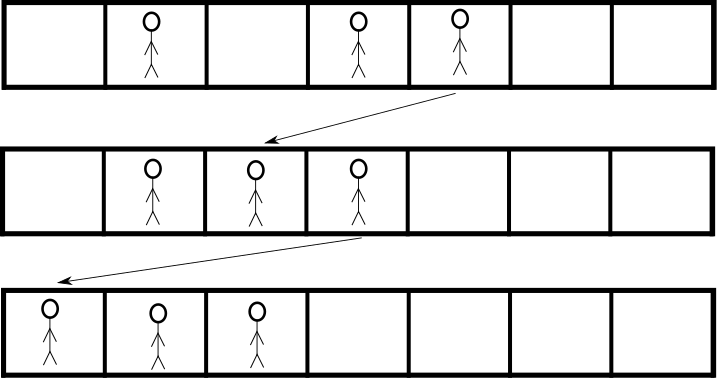
\includegraphics[width=0.3\textwidth]{sample.png}
  \caption{Illustration of the example}
\end{figure}

\section*{Task}
Your task is to compute something or other. You will implement the function \texttt{invigilation(N, H, X, Y, Z)}.

\begin{itemize}
  \item \texttt{invigilation(N, H, X, Y, Z)} - this function will be called exactly once by the judge.
  \begin{itemize}
    \item \texttt{N}: the number of points of the wall.
    \item \texttt{H}: the Y position of the highway.
    \item \texttt{X}: an array with $N$ elements. \texttt{X[i]} ($0 \le i < N$) contains the X coordinate of the $i$:th point of the wall.
    \item \texttt{Y}: an array with $N$ elements. \texttt{Y[i]} ($0 \le i < N$) contains the Y coordinate of the $i$:th point of the wall.
    \item \texttt{Z}: an array with $N$ elements. \texttt{Y[i]} ($0 \le i < N$) is 1 if there is a tower on the $i$:th point of the wall, or 0 if not.
    \item $3 \le N \le 10^5, 1 \le H \le 10^6$
    \item $0 \le X[i] \le 10^6, 0 \le Y[i] < H$
    \item \texttt{Y[0]} = \texttt{Y[N-1]} = 0
    \item $X$ is strictly increasing.
    \item The function should return the minimum number of cameras Gargamal needs to use.
  \end{itemize}
\end{itemize}

\section*{Subtasks}
The problem consists of a number of subtasks. Each subtask gives some amount of points, and to pass
the subtask you must pass all the test cases in the subtask.

\begin{tabular}{|l|l|l|}
  \hline
  \textbf{Subtask} & \textbf{Points} & \textbf{Limits} \\ \hline
  1 & 30 & $1 \le N \le 1\,000$ \\ \hline
  2 & 30 & $1 \le N \le 100\,000$, the wall will be convex upward. \\ \hline
  6 & 40 & $1 \le N \le 100\,000$ \\ \hline
\end{tabular}

The wall being convex upward means that for any two consecutive line segments of the wall, the slope of the second will be smaller than or equal to slope of the first.
I.e., the following inequality will hold:

$(Y[i+2] - Y[i+1]) / (X[i+2] - X[i+1]) \le (Y[i+1] - Y[i]) / (X[i+1] - X[i])$

\section*{Input format}
The sample judge reads input in the following format:

\begin{itemize}
  \item line $1$: \texttt{N H}
  \item line $i = 2 \dots N+1$: \texttt{X[i-2] Y[i-2] Z[i-2]}
\end{itemize}

\section*{Output format}
The sample judge will first write a single line with the return value of \texttt{invigilation(N, H, X, Y, Z)}.
